\chapter{Спектральная диагностика~низкотемпературной плазмы газового разряда}
%\chapter{СПЕКТРАЛЬНАЯ ДИАГНОСТИКА НИЗКОТЕМПЕРАТУРНОЙ ПЛАЗМЫ ГАЗОВОГО РАЗРЯДА}
\label{cha:ch_1}
\section{Кинетика заселения возбужденных атомных состояний в плазме}
Спектры излучения газоразрядной плазмы определяются населенностью \math{N_j}$ соответствующих возбужденных атомных уровней \math{E_j}$.
Тогда интенсивность соответствующей атомной спектральной линии составит:
\begin{equation}
    I_{ji} = A_{ji}h\nu_{ji}⋅N_j
\end{equation}
где \math{A_{ji}}$  - коэффициент Эйнштейна для перехода \math{j → i}$, \math{N_j}$ - населенность возбужденного уровня \math{j}$.

Таким образом, задача спектральной диагностики плазмы сводится к построению теоретических моделей, связывающих
параметры плазмы (в первую очередь, концентрации электронов \math{n_e}$ и их температуру \math{T_e}$) с интенсивностями спектральных
линий \math{I_{ji}}$. Выбор той или иной модели зависит от параметров плазмы: ее химического состава, плотности,
степени ионизации и равновесности. В данной работе экспериментально и теоретически исследуется стационарная сильно
неравновесная плазма положительного столба слаботочного газового разряда постоянного тока (\math{I_{DC}~=~1}$~мА)
в неоне при давлении \math{P~=~60}$~Па, причем степень ионизации плазмы α очень мала (\math{\alpha~\sim~10^{-8}}$).
Выбор этих параметров обуславливается практическим случаем, рассматриваемым в этой работе.
\begin{figure}[t]
    \begin{center}
         \subfloat[\label{sub:fig11a}]{
           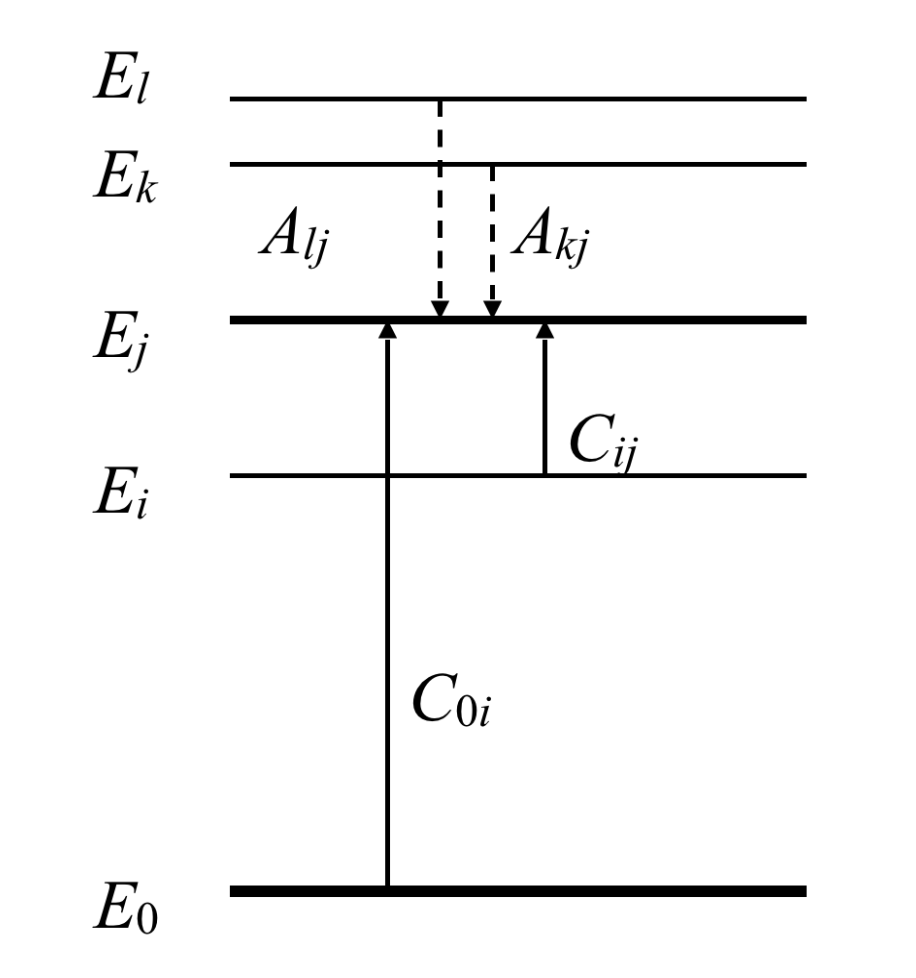
\includegraphics[width=0.35\textwidth]{figures/fig11a}
         }
         \hspace{0.05\columnwidth}
         \subfloat[\label{sub:fig11b}]{
           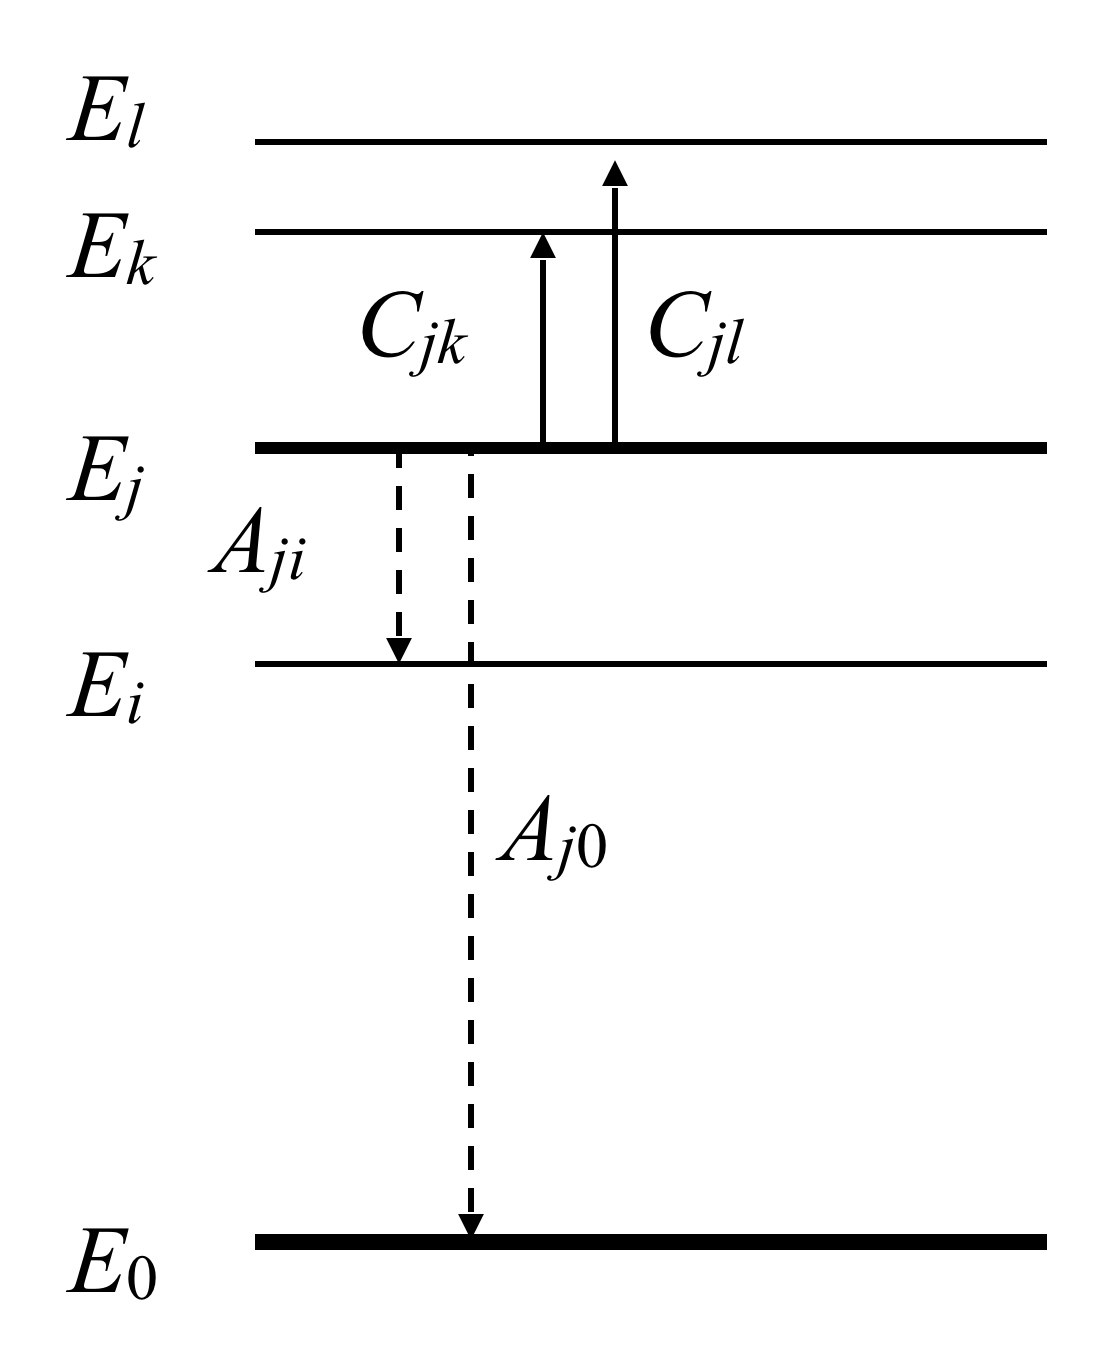
\includegraphics[width=0.305\textwidth]{figures/fig11b}
         }
         \caption{Схема основных процессов уровня: \pt(a) заселение, \pt(b) расселение.}
         \label{fig:fig11}
    \end{center}
\end{figure}

Населенность \math{N_j}$ уровня \math{E_j}$ в стационарном случае определяется балансом процессов его заселения
и расселения. Схема основных процессов заселения уровня \math{E_j}$ представлена на рис.~\ref{fig:fig11}~\subref{sub:fig11a}.
Основным процессом заселения рассматриваемого уровня \math{E_j}$ является его заселение прямым
электронным переходом с основного состояния \math{E_0}$ и с метастабильного \math{E_i}$.

Скорости процессов \math{C_{0j}}$ и \math{C_{ij}}$ определяются соотношениями:
\begin{equation}C_{0j} = \sqrt{2 \over m_e} \int_{E_j}^{\infty} \sigma_{0j}(E) f_e(E) \sqrt{E} dE\end{equation}
и
\begin{equation}C_{ij} = \sqrt{2 \over m_e} \int_{E_j - E_i}^{\infty} \sigma_{ij}(E) f_e(E) \sqrt{E} dE\end{equation}
соответственно, где …

Сечения \math{\sigma_{0j}(E)}$ и \math{\sigma_{ij}(E)}$ расчетные и экспериментальные, можно найти в литературе
или базе данных NIST [ССЫЛКА НА ИСТОЧНИК]. Типичный вид сечений представлен на рис. \ref{fig:fig12}.
Что касается вида ФРЭ, то она сильно зависит от параметров плазмы. При высоких давлениях ФРЭ приближается
к максвелловской функции. Однако, при низких давлениях плазма сильно неравновесна, и вид функции ФРЭ должен
быть определен дополнительными методами. Кроме столкновительного заселения уровень \math{E_j}$ заселяется
также путем радиационного распада верхних \math{k}$-уровней \math{E_k~>~E_j}$ cо скоростью \math{A_{kj}}$ при \math{k > j}$.
Значения \math{A_{kj}}$ также табулированы в базе данных NIST.
\begin{figure}[t]
  \centering
  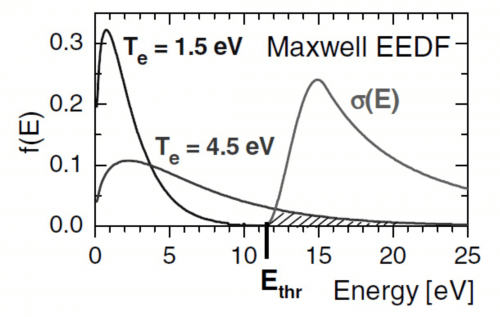
\includegraphics[width=8cm]{figures/fig12}
  \caption{Типичный вид сечения \math{\sigma}$ и максвелловской ФРЭ. \math{T_e}$ - температура электронов, \math{E_{thr}}$ - пороговая энергия..}
  \label{fig:fig12}
\end{figure}

Схема основных процессов расселения уровня \math{E_j}$ представлена на рис.~\ref{fig:fig11}~\subref{sub:fig11b}.
Этими процессами также являются явления спонтанного распада возбужденных уровней и столкновительные процессы,
индуцированные свободными электронами.

Приравняв скорости заселения и расселения уровня \math{E_j}$, мы получим уравнение относительно ФРЭ \math{f_e(E)}$.
Это уравнение является некорректной задачей и для ее решения необходимы дополнительные данные о виде ФРЭ.
Эти данные могут быть получены путем решения кинетического уравнения Больцмана для соответствующих условий.

\section{Уравнение Больцмана для ФРЭ в положительном столбе газового разряда постоянного тока.}

Газовые разряды представляют собой крайне неравновесную систему, в которой средняя энергия электронов (температура)
на два порядка превышает температуру газа. Функция распределения электронов (ФРЭ) характеризуется нагревом
электронов электромагнитными полями и столкновениями их с нейтральными атомами, почти во всех случаях это распределение
отклоняется от равновесного (Максвелловского). Решение кинетического уравнения Больцмана для ФРЭ является
важнейшей задачей для точного моделирования плазмы, так как многие явления невозможно правильно понять
без кинетического анализа. Уравнение Больцмана существенно можно упростить из-за большого различия масс электронов и атомов.
В силу данного различия, затухание энергии электронов в упругих столкновениях с атомами происходит гораздо медленнее,
чем затухание импульса электронов (\math{m_e \ll M_a}$). Как следствие, ФРЭ в скоростном пространстве может быть представлена как сумма
большой изотропной \math{f_0}$ и малой анизотропной частей \math{f_1}$.

Выделяют три существенно различных случая. Первый случай, когда величины \math{P L \gg 1}$ и \math{{E P} \ll 1}$, где
\math{P}$ - давление газа, \math{L}$ - характерный размер плазмы, \math{E}$ - электрическое поле, а
пространственные градиенты \math{f_0}$ и \math{f_1}$ малы и определены локальными значениями электрического поля,
электронной плотности и составом плазмы. Тогда электроны могут быть описаны уравнениями жидкости с коэффициентами переноса,
полученными из локальной (не Максвелловской) ФРЭ. Обычно через уравнение Больцмана решают задачу нахождения
коэффициентов переноса и скоростей протекания реакции для данного приближения.

Второй случай соответствует столкновительной плазме, где характерный размер плазмы \math{L}$ значительно больше средней длины
свободного пробега электронов \math{\lambda}$, но сравним с длиной релаксации энергии электрона \math{\lambda_\epsilon}$.
В этом нелокальном режиме изотропная часть ФРЭ \math{f_0}$ в заданной точке зависит не только от электрических полей в этой точке,
но и от свойств плазмы в окрестности точки размера (эффект памяти), а анизотропная часть \math{f_1}$ является лишь функцией
электрического поля \math{E}$. В этом столкновительном режиме плазма не может быть описана гидродинамикой.

В третьем случае, при дальнейшем уменьшении \math{P L}$, средняя длина свободного пробега электрона будет сравнима c характерным размером плазмы
(\math{\lambda \sim L)$. В этом почти бесстолкновительном случае анизотропная часть в точке определяется не только
значением напряженности электрического поля в этой точке, но и профилем электрического поля вдоль траектории электрона.
В результате локальная зависимость между плотностью тока и электрическим полем (закон Ома) становится недействительной \cite{Kolobov}.

Плазма тлеющего разряда низкого давления имеет сильно неравновесный характер. Рождение заряженных частиц происходит
преимущественно в объемных процессах, а гибель на стенках разрядной камеры. Энергию электроны приобретают,
разгоняясь в электрическом поле, а теряют в упругих и неупругих столкновениях. Количественное описание этих процессов
возможно только на кинетическом уровне \cite{Zobnin}.

В данной работе положительный столб газового разряда находится под низким давлением порядка 60~Па и имеет диаметр трубки 30~мм (см. раздел \ref{sec:sec_31}),
а значит для описания кинетических процессов с помощью уравнения Больцмана необходимо пользоваться почти бесстолкновительным приближением.

Кинетическое уравнение Больцмана представляет собой интегродифференциальное уравнение, описывающее эволюцию функции
распределения частиц в шестимерном (6-D) фазовом пространстве. Данное уравнение было выведено Людвигом Больцманом в 1872 г.
Оно до сих пор остается основой кинетической теории газов и оказывается плодотворным не только для исследования
классических газов, которые имел в виду Больцман, но - при соответствующем обращении - и для излучения переноса
электронов в твердых телах и плазме \cite{Cherchin'yani}. В общем виде оно выглядит следующим образом (также данное
уравнение называют уравнением Власова):

\begin{equation}
    {\partial f_e \over \partial t} + (\vec{v}, \vec{\Delta}_r) f_e + (\vec{a}, \vec{\Delta}_v) f_e = I
    \label{eq:vlasov}
\end{equation}
где \math{f_e = f_e(\vec{r}, \vec{v}, t)}$~--~функция распределения электронов,
\math{\vec{r}}$~--~вектор положения в физическом пространстве, \math{\vec{v}}$~--~вектор скорости,
\math{\vec{a}}$~--~вектор ускорения, \math{t}$~--~время, \math{I}$~--~интеграл столкновений,
является интегральным оператором в пространстве скоростей, в котором должны быть учтены все элементарные процессы
с участием электронов, приводящие к изменению их числа в объеме \math{dx dy dz dv_x dv_y dv_z}$ фазового пространства.

Решение этого интегродифференциального нелинейного уравнения сопряжено с огромными математическими трудностями и
поэтому всегда проводится с привлечением ряда серьезных упрощений. Многие сотни журнальных публикаций посвящены
конкретным расчетам \math{f(V)}$ в различных условиях, однако среди них далеко не всегда удается найти требуемое.
Вместе с тем экспериментатору часто приходится хотя бы оценить ожидаемый вид \math{f(V)}$ в условиях его работы \cite{Kolesnikov}.

%{e \over m_e} \vec{E}

Для слабоионизированной плазмы столкновения электронов с нейтралами обычно преобладают над столкновениями между
заряженными частицами. Из-за разницы масс электрона и атома (\math{m_e \ll M_a}$) интеграл столкновения
для упругих взаимодействий электронов с тяжелыми нейтралами может быть записан в так называемой форме Лоренцевского газа
\cite{Kolobov}:
\begin{equation}
    I_{el} = - {1 \over v^2} {\partial \over \partial v} v^2 \Gamma - N v \int_{S^2} \sigma (v, |\Omega - \Omega^{'}|) [f(v, \Omega^{'}) - f(v, \Omega)] d \Omega
    \label{eq:lorentz}
\end{equation}
где \math{\Omega}$~--~телесный угол фазового пространства скоростей на единичной сфере \math{S^2}$ (\math{\vec{v} = v \Omega}$),
\math{\sigma}$~--~сечение столкновения, \math{N}$~--~концентрация атомов газа, поток \math{\Gamma}$ задается следующим образом:
\begin{equation}
    \Gamma = - {\delta \nu \over 2} \big{(} v f + {T \over m} {\partial f \over \partial v} \big{)}
\end{equation}
где \math{T}$~--~температура газа, \math{\nu}$~--~транспортная частота столкновений и \math{\delta = (2m / M)}$~--~
средняя доля энергии, которая теряется электронами в упругих столкновений. Первое слагаемое в (\ref{eq:lorentz}) мало, оно
отвечает за обмен энергиями между электронами и нейтралами. Второе слагаемое в (\ref{eq:lorentz}) описывает столкновения
электронов с бесконечно тяжелыми частицами, которые в основном не меняют свою энергию, а лишь изотропно меняют
распределение электронов. Таким образом для того, чтобы ФРЭ пришла в равновесие с полем необходимо, чтобы прошло время
намного превышающе \math{({\nu m / M})^{-1}}$ \cite{Tsendin}.

Таким образом, для почти бесстолкновительного случая в качестве приближения ФРЭ для решения уравнения Власова (\ref{eq:vlasov}) можно
использовать достаточно распространенное двухчленное приближение:
\begin{equation}f_e(\vec{r}, \vec{v}, t) = f_0(\vec{r}, \vec{v}, t) + { \vec{v} \over v} \vec{f_1} (\vec{r}, \vec{v}, t)\end{equation}
где \math{f_1}$ отвечает за анизотропию.

Подставив это приближение в уравнение (\ref{eq:vlasov}) и усреднив по направлениям скоростей (в силу их изотропности из-за
столкновений с тяжелыми частицами), получим следующую систему уравнений, которую называют системой
Давыдова-Эллиса \cite{Kolobov}:
\begin{equation}
 \begin{cases}
  {\partial \vec{f_1} \over \partial t} + \nu \vec{f_1} = - v \nabla f_0 - {e \vec{E} \over m} {\partial f_0 \over \partial v},
   \\
   {\partial f_0 \over \partial t} + {v \over 3} div(\vec{f_1}) + {1 \over 3v^2} {\partial \over \partial v } ({ v^2 e \vec{E} \over m} \vec{f_1} ) = S_0
 \end{cases}
 \label{eq:davydov-ellis}
\end{equation}
Здесь \math{e}$~--~модуль заряда электрона, \math{m}$~--~масса электрона, \math{S_0}$ —  часть интеграла столкновений,
отвечающая за упругие и неупругие электрон-атомные столкновения и электрон-электронные взаимодействия

В левой части первого уравнения системы (\ref{eq:davydov-ellis}) можно пренебречь слагаемым
{\partial \vec{f_1} \over \partial t}$, так как мы рассматриваем выход ФРЭ на стационарный уровень во времени,
где анизотропические эффекты уже не имеют значения.

Перейдя от скоростей к энергиям \math{v = \sqrt{2 \epsilon \over m}}$,
\math{{\partial f(v) \over \partial v}  = {\partial f(\epsilon) \over \partial \epsilon} \sqrt{2 \epsilon m}}$
в системе Давыдова-Эллиса (\ref{eq:davydov-ellis}) и подставив выражение для \math{\vec{f_1}}$ в нижнее уравнение, получим:
\begin{equation}
    \begin{gathered}
        \sqrt{\epsilon} {\partial f_0 \over \partial t} = \sqrt{2 \over m} \big{[} S_0 + {\partial \over \partial \epsilon}
        [\epsilon^{3 \over 2} ({2 m \over M} \nu f_0 + {e^2 (\vec{E}, \vec{E}) \over 3 \nu} {\partial f_0 \over \partial \epsilon})] \big{]}
    \end{gathered}
\end{equation}
где \math{M}$ - масса молекулы неона.

Поскольку столб газового разряда геометрически представляет собой продольную трубку,
вдоль которой течет ток, то модуль электрического поля равен продольной составляющей \math{|\vec{E}|} = E_z}$, также его
называют осевым электрическим полем. Подставив значение транспортной частоты \math{\nu = N_g \sigma_t \sqrt{\epsilon}}$ и
осевого электрического поля, а также выполнив незначительные преобразования (в том числе переобозначение \math{f_0 = f}$), получим:
\begin{equation}
    \begin{gathered}
        \sqrt{\epsilon} {\partial f \over \partial t } = \sqrt{2 \over m} \big{[} S_0 + 2 {m \over M} N_g
        {\partial \over \partial \epsilon} \big{[} \sigma_t \epsilon^2 f \big{]}
        + {e^2 E_z^2 \over 3 N_g} {\partial \over \partial \epsilon} \big{[} {\epsilon \over \sigma_t}
        {\partial f \over \partial \epsilon} \big{]} \big{]}
    \end{gathered}
    \label{eq:main_eq}
\end{equation}

Вид \math{S_0}$ зависит от того, какие взаимодействия с электронами учитываются.
В данной работе использовался следующий вид \math{S_0}$, записанный в дискретной форме:
\begin{equation}
    S_0 = \sum_k \big{[} \sqrt{\epsilon + \epsilon_k} \nu_k (\epsilon + \epsilon_k)f(\epsilon + \epsilon_k) - \sqrt{\epsilon} \nu_k(\epsilon)f(\epsilon) \big{]}
    \label{eq:S_0}
\end{equation}
суммирование проводится по всем верхним энергетическим уровням k, которые больше аргумента функции \math{\epsilon}$,
частота столкновения k-уровня записывается так \math{\nu_k(\epsilon) = \sigma_k(\epsilon)N_g\sqrt{\epsilon}}$,
\math{N_g}$ - концентрация атомов.

В почти бесстолкновительном случае для поиска концентрации атомов Ne \math{N_g}$ можно воспользоваться уравнением состояния идеального газа,
поскольку атомы между собой почти не взаимодействуют:
\begin{equation}
    N_g = {P \over k_b T}
    \label{eq:concentration}
\end{equation}
где \math{P}$~--~давление газа 60~Па; \math{k_b}$~--~постоянная Больцмана; \math{T}$~--~температура газа 294~K.

\section{Решение уравнения Больцмана и результаты}

В данном подразделе описываются численные подходы, алгоритмы и аппроксимации необходимые для нахождения численного решения
функций распределения электронов для различных осевых электрических полей в диапазоне \math{1 \le E_z \le 10}$~В/см,
которые задаются параметрически.

Рассматривается задача решения разностной схемы относительно \math{f}$ на основе уравнений (\ref{eq:main_eq}) и (\ref{eq:S_0}).
Данная задача является краевой: вероятность нахождения электронов при бесконечно большой энергии стремится к нулю, а
вероятность нахождения электронов с положительном энергией максимальна, т.е. первая производная ФРЭ по энергии в нуле
будет равна нулю. Имеем следующие граничные условия:
\begin{equation}
    \begin{cases}
        {d f \over d \epsilon}(0) = 0
        \\
        f(\infty) = 0
    \end{cases}
    \label{eq:borders}
\end{equation}

Если обратить внимание на уравнения (\ref{eq:main_eq}) и (\ref{eq:S_0}), то становится ясно, что аналитически выразить
\math{f}$ для явного построения разностной схемы невозможно, поскольку в (\ref{eq:S_0}) \math{f}$ принимает значения для
аргументов, отличных от \math{\epsilon}$. Следовательно, при данной трактовки задачи необходимо получить дополнительное граничное
условие для каждого элемента суммирования \math{\epsilon_k}$, например с помощью двухточечной краевой задачи (метод стрельбы),
и сводить исходную задачу к задаче Коши. Это довольно сложный подход, более того, нет необходимости для каждого момента времени
решать задачу Коши, поскольку нас интересует ФРЭ при выходе на стационарный уровень во времени, а не при сложных переходных процессах.

Предполагается, что функция распределения электронов при заданном электрическом поле выйдет на стационарый уровень: из-за
невысоких полей данное предположение более, чем разумно. Поэтому будем высчитывать с помощью метода временной эволюции
относительную разницу ФРЭ между итерациями по времени и смотреть, если относительное изменение достаточно незначительно, то ФРЭ вышла
на стационарный уровень; далее решается краевая задача с граничными условиями (\ref{eq:borders}).
Построим разностную схему для данного подхода:
\begin{equation}
\begin{small}
    \begin{gathered}
        f^n(\epsilon) = f^{n-1}(\epsilon) + \Delta t \sqrt{2 \over m \cdot \epsilon}
        \Big{[} N_g \sum_k
            \big{[}
                F^{n-1}_k (\epsilon + \epsilon_k) - F^{n-1}_k (\epsilon)
            \big{]} + \\
        {2 m N_g \over M}
            \big{[}
                {F^{n-1}_t(\epsilon + \Delta \epsilon) \cdot (\epsilon + \Delta \epsilon) -
                F^{n-1}_t(\epsilon - \Delta \epsilon) \cdot (\epsilon - \Delta \epsilon)  \over 2 \Delta \epsilon }
            \big{]} + \\
        {1 \over \Delta \epsilon} \cdot {e^2 E_z^2 \over 3 N_g} \cdot
            \big{[}
                {\epsilon + { \Delta \epsilon \over 2 } \over  \sigma_t(\epsilon + { \Delta \epsilon \over 2 })} \cdot
                {f^{n-1}(\epsilon + \Delta \epsilon) - f^{n-1}(\epsilon) \over \Delta \epsilon } -
                {\epsilon - { \Delta \epsilon \over 2 } \over  \sigma_t(\epsilon - { \Delta \epsilon \over 2 })} \cdot
                {f^{n-1}(\epsilon) - f^{n-1}(\epsilon - \Delta \epsilon) \over \Delta \epsilon }
            \big{]}
        \Big{]}
    \end{gathered}
\end{small}
\label{eq:razh_scheme}
\end{equation}
где \math{\epsilon}$~--~энергия в~эВ; \math{\Delta \epsilon}$~--~шаг по энергии в~эВ;
\math{f^n (\epsilon)}$~--~ФРЭ с энергией \math{\epsilon}$, имеющая \math{n}$-й шаг по времени;
\math{\sigma_t (\epsilon)}$~--~транспортное сечение упругого рассеяния;
\math{\sigma_k (\epsilon)}$~--~сечение неупругих столкновений для k-уровня;
\math{N_g}$~--~концентрация атомов \math{Ne}$ в см^{-3}; \math{M}$~--~масса молекулы Ne в граммах;
\math{m}$~--~масса электрона в граммах; \math{e}$~--~заряд электрона в Кл;
\math{k}$~--~итератор суммирования по всем энергиям верхних уровней, значения которых больше \math{\epsilon}$;
\math{E_z}$~--~осевое электрическое поле, которое задается параметрически в диапазоне \math{1 \le E_z \le 10}$~В/см с шагом \math{0.1}$~В/см;
для удобства записи выполнена замена
\math{F^n_i}(\epsilon) = f^n(\epsilon) \cdot \sigma_i(\epsilon) \cdot \epsilon }$, где \math{i}$ обозначает природу сечения.

\begin{figure}[t]
  \centering
  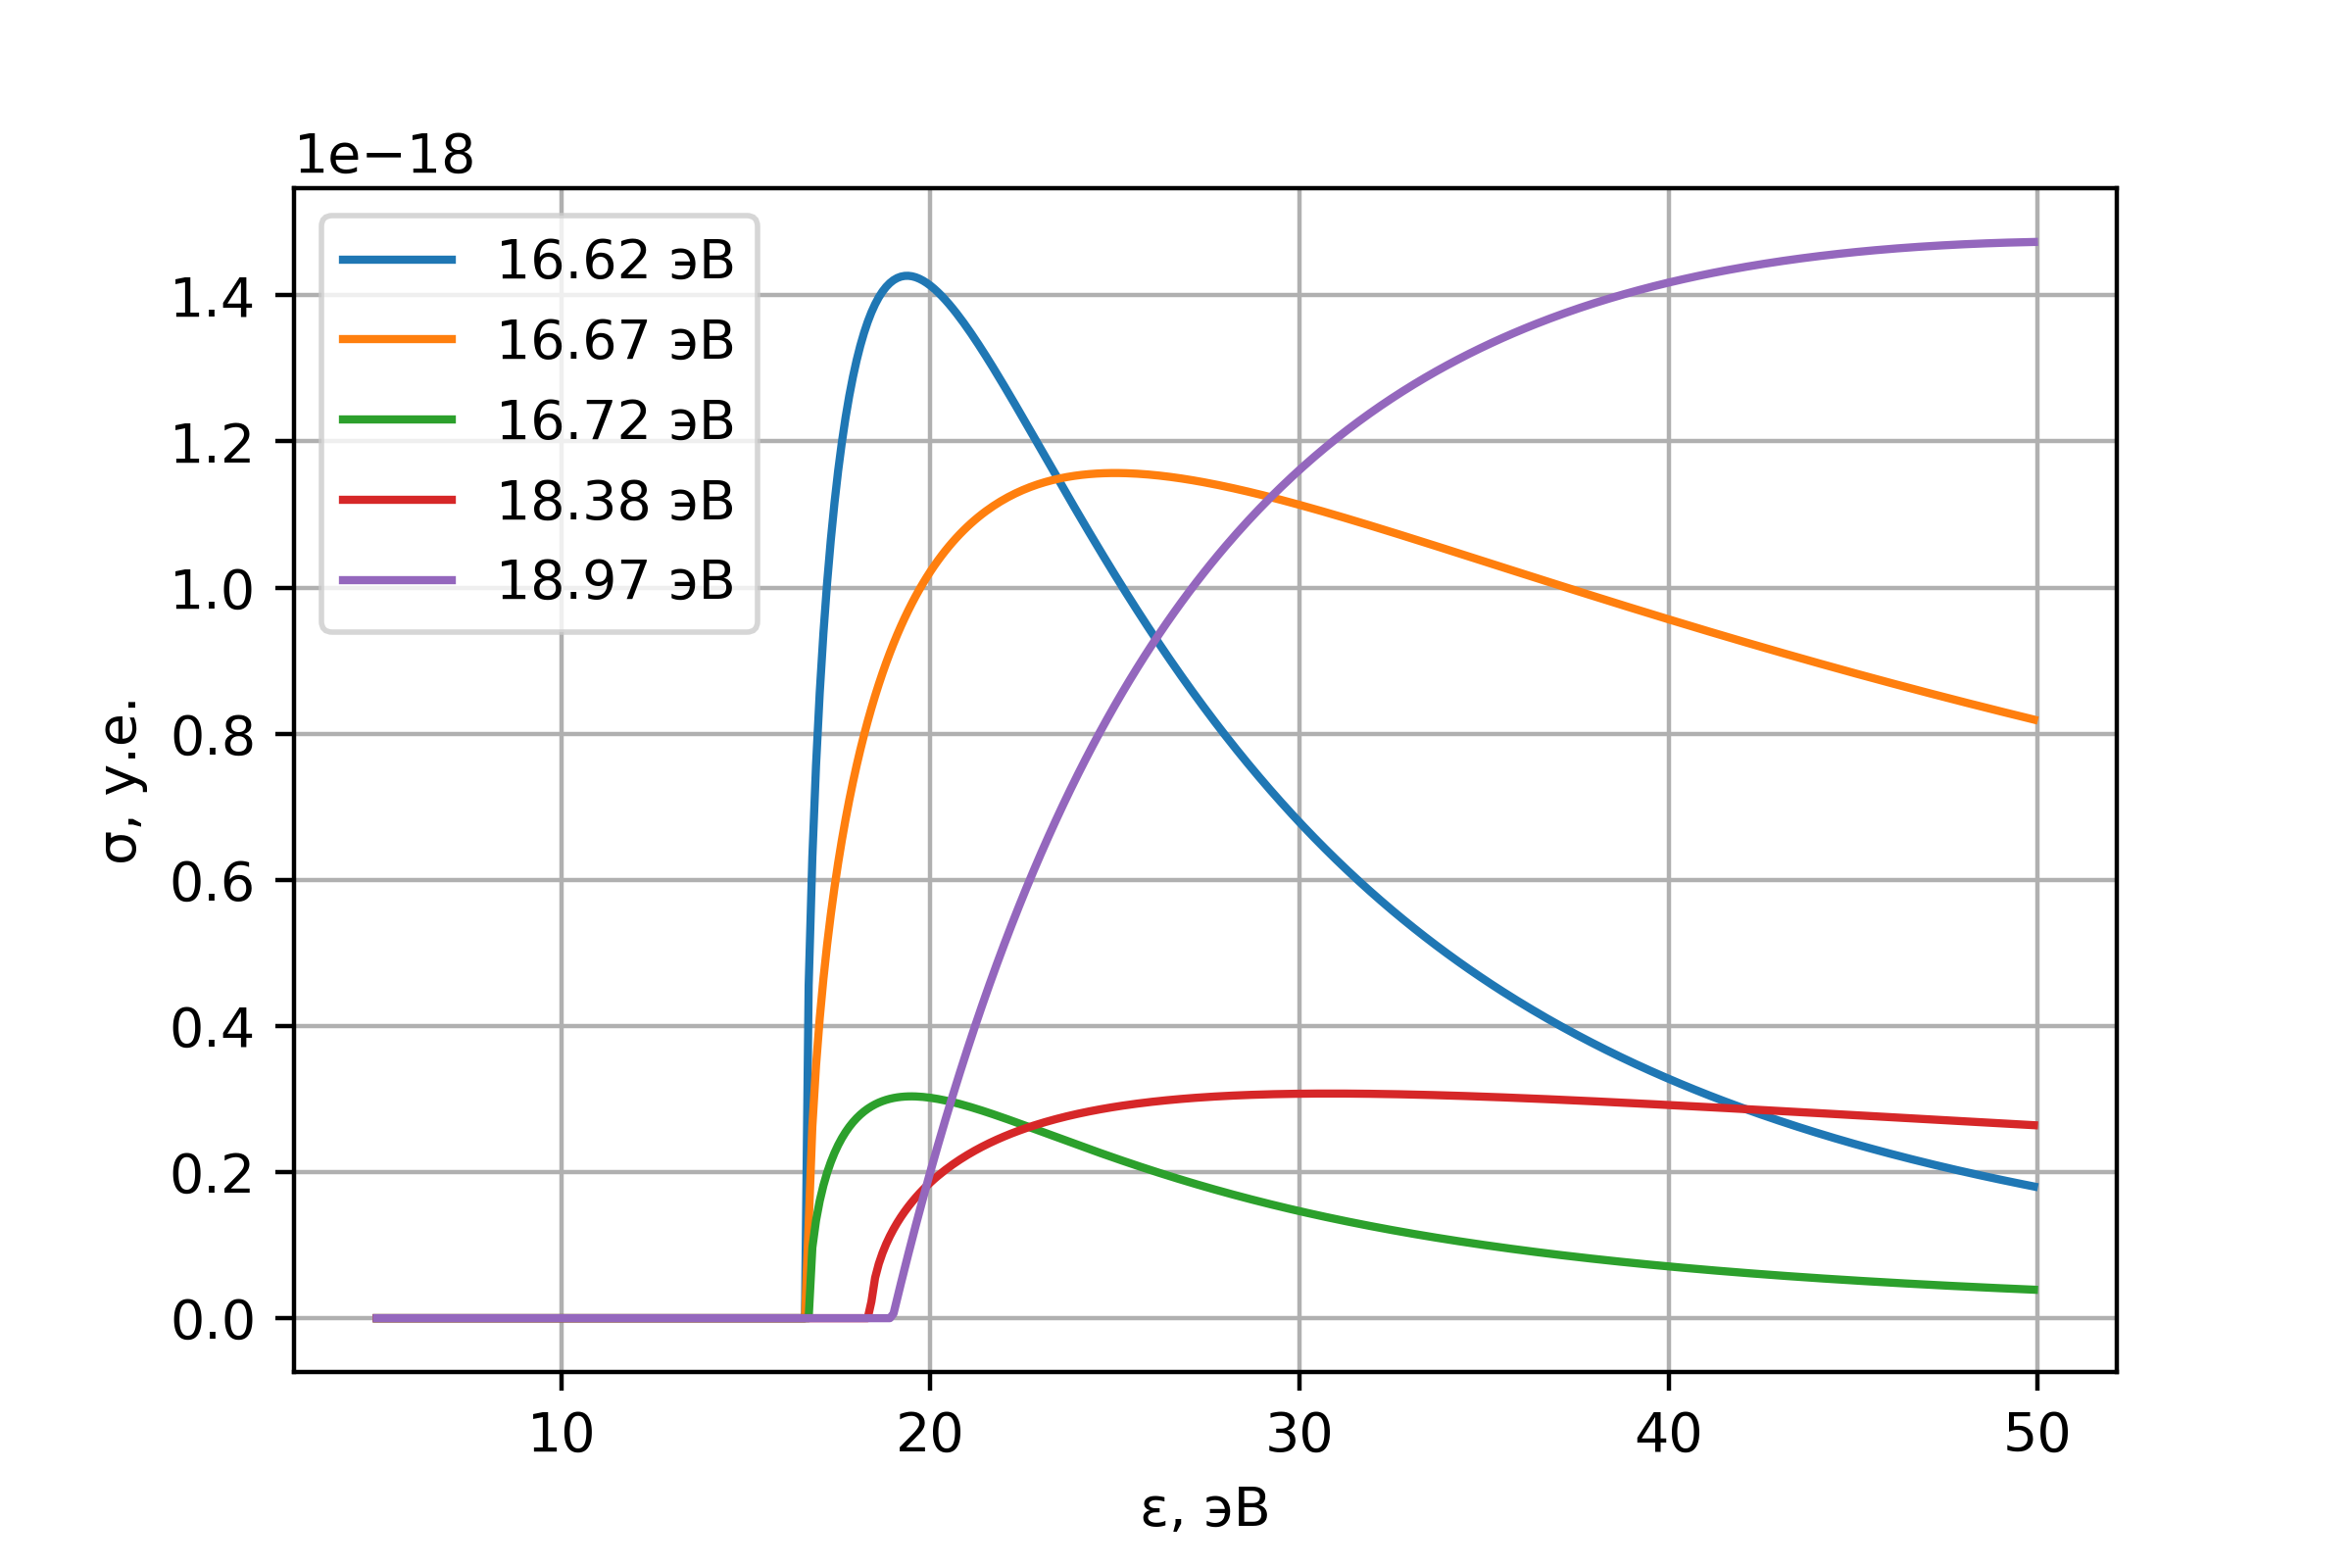
\includegraphics[width=15cm]{figures/fig13}
  \caption{Графическое представление некоторых аппроксимаций сечений рассеяния для различных энергетических уровней.}
  \label{fig:fig13}
\end{figure}

На языке разностной схемы граничные условия (\ref{eq:borders}) будут выглядить следующим образом:
\begin{equation}
    \begin{cases}
        f^n_0 = f^n_1
        \\
        f^{n}_K = 0
    \end{cases}
    \label{eq:razn_borders}
\end{equation}
где K~--~максимальное количество шагов по энергии, в рамках данной задачи энергию равной 50~эВ можно считать уже бесконечно большой.
То есть при шаге \math{\Delta \epsilon = 0.1}$~эВ максимальное количество шагов по энергии будет \math{K = 500}$.

В качестве начальных условий при \math{t = 0}$ для первого вычисления ФРЭ (при \math{E = 1}$~В/см) предлагается взять
распределение Больцмана:
\begin{equation}
    f^0 (\epsilon) = 0.7 \cdot e^{- {\epsilon \over 6}}
    \label{eq:start_condition}
\end{equation}

Данная функция намного ближе к итоговому решению, чем прямая, а значит для сходимости нужно будет выполнить меньше итераций
по времени: чем приближеннее возьмем начальное условие, тем быстрее наступит стационарный уровень. По данным соображениям
для подсчета ФРЭ для следующих полей удобнее всего брать за начальные условия результаты предыдущего расчета.

В данной работе использовались следующие аналитические аппроксимации для сечений элементарных процессов, полученные частично из
\cite{Zobnin}, частично из последних трудов Зобнина~А.~В.:
\begin{figure}[t]
  \centering
  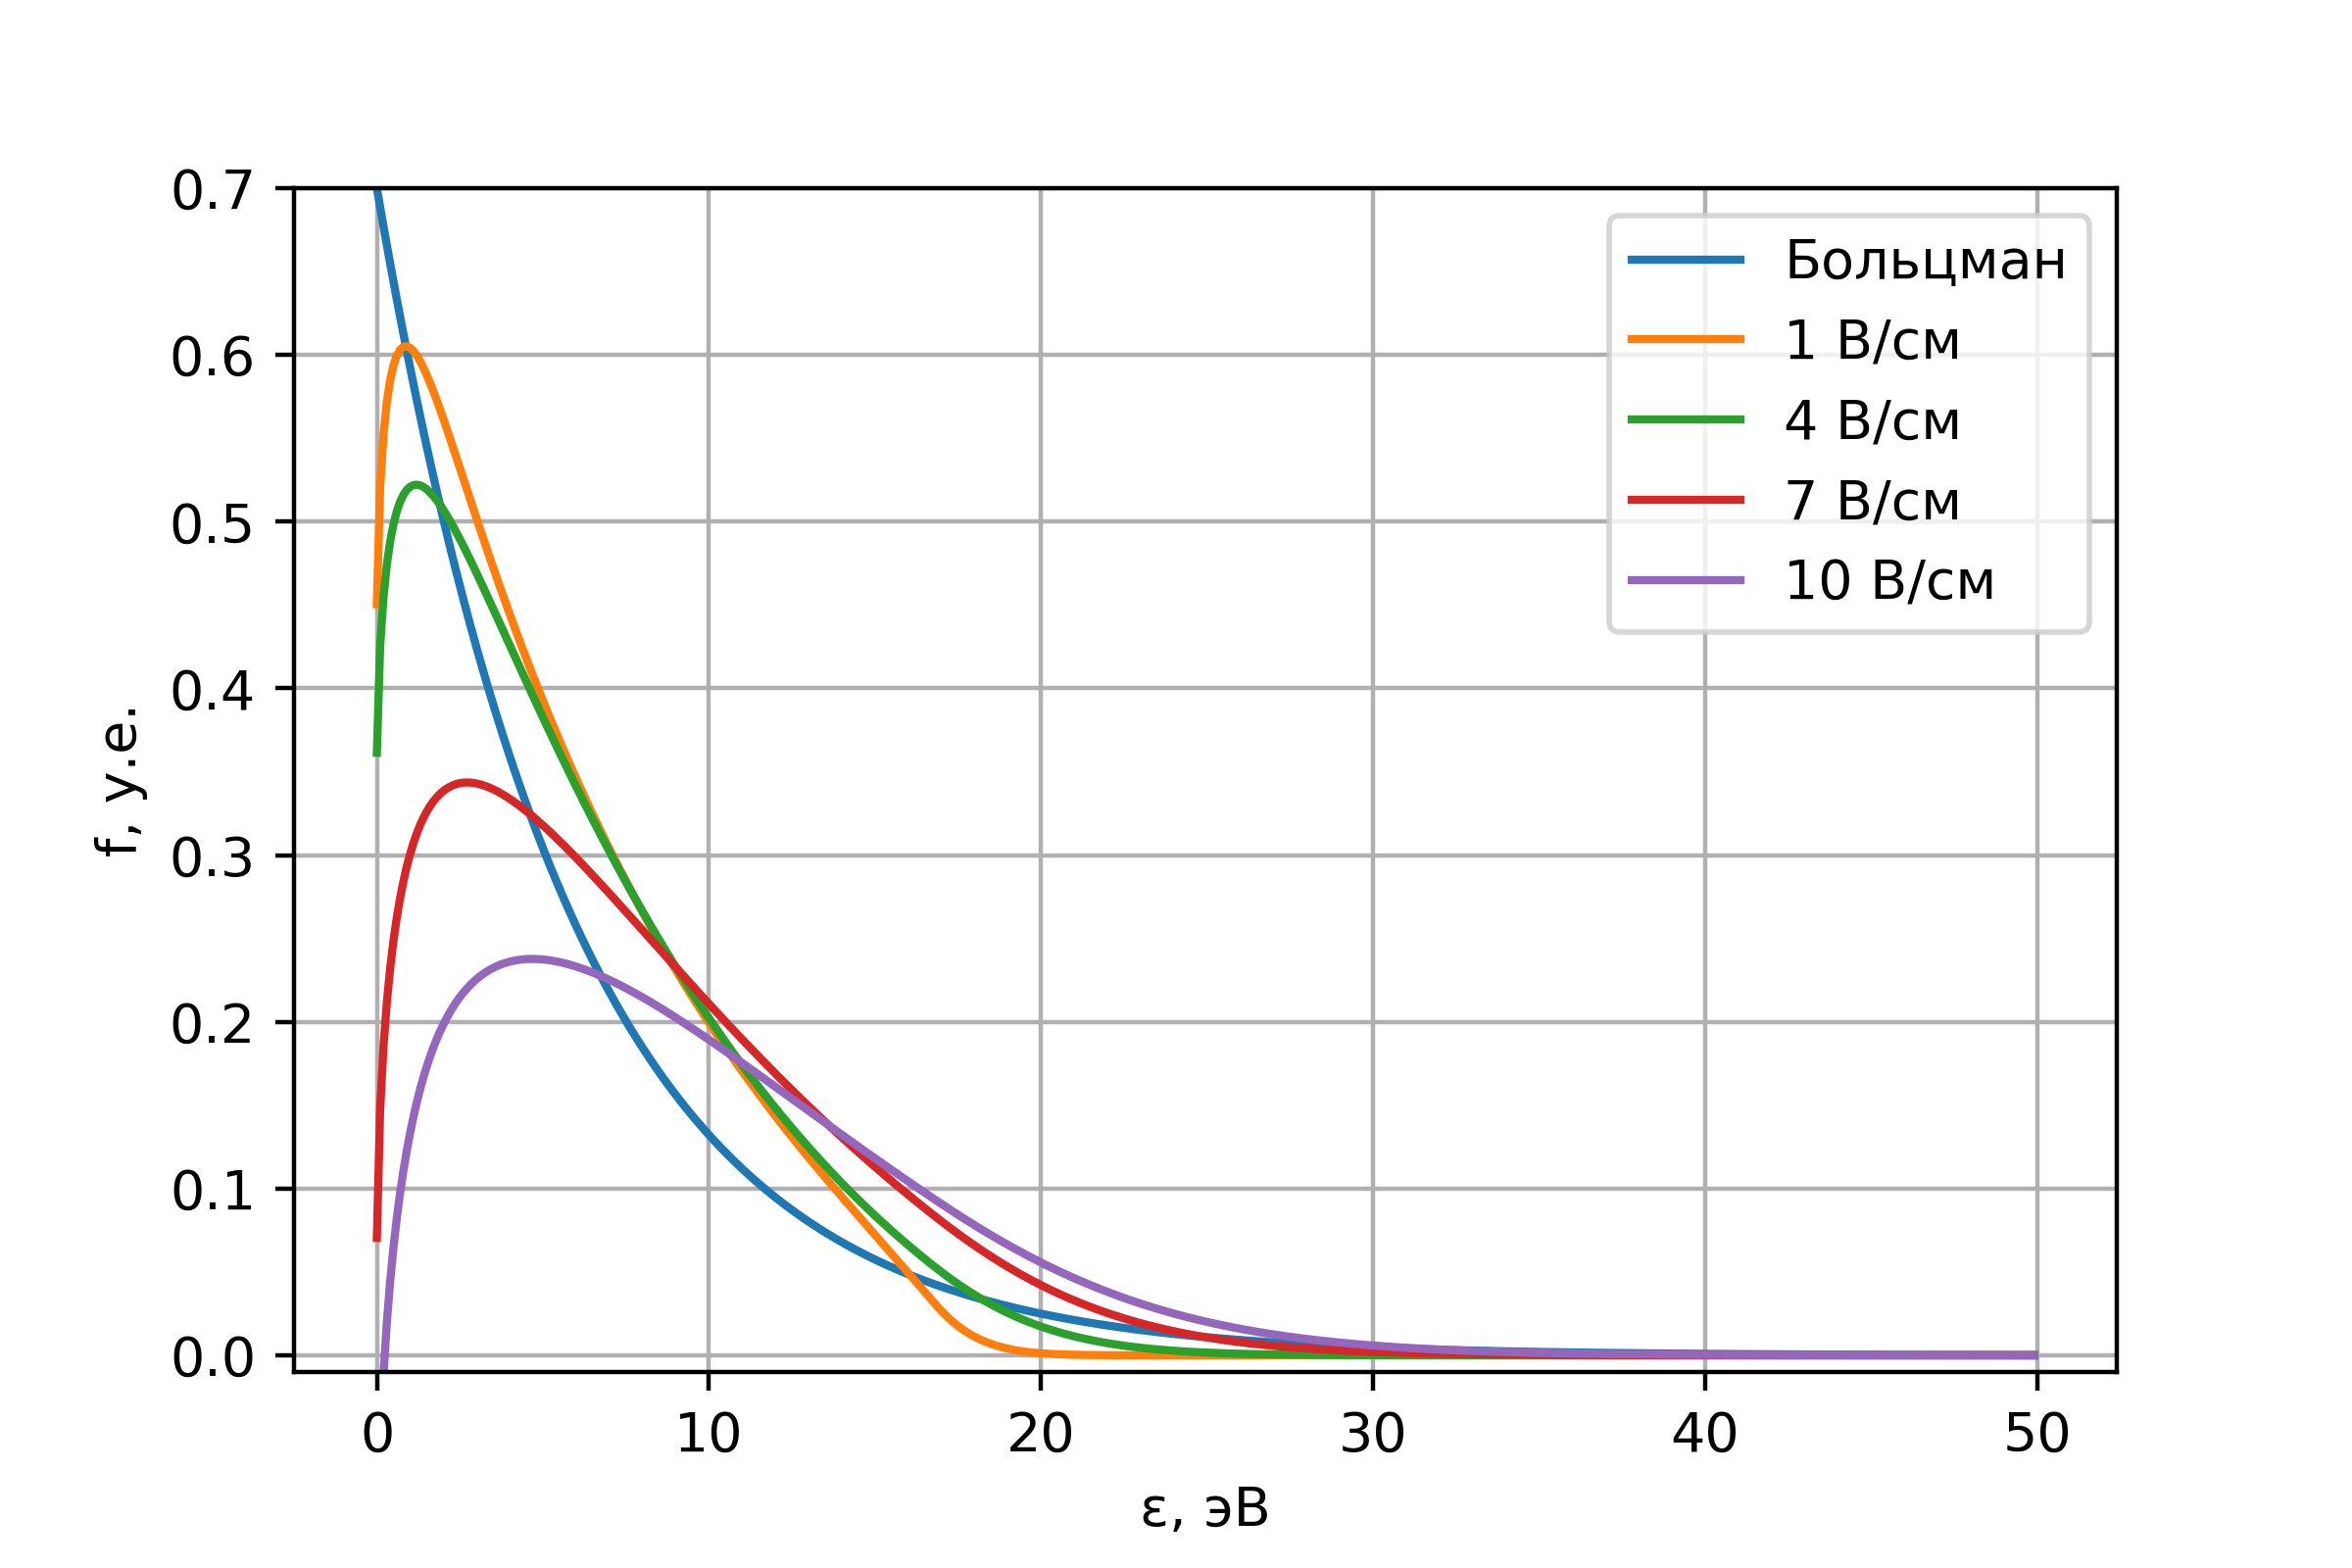
\includegraphics[width=15cm]{figures/fig14}
  \caption{Зависимость расчетной функции распределения электронов от энергии и осевого электрического поля,
  заданного параметрически для некоторых значений; также нанесено распределение Больцмана, которое использовалось в качестве
  начального условия (\ref{eq:start_condition}).}
  \label{fig:fig14}
\end{figure}
\begin{equation*}
    \sigma_t(\epsilon) = \begin{cases}
    \big{[}
        2.56 + 0.57 \cdot \ln
        \big{(}
            0.02 + {\epsilon \over 5.5 + \epsilon^2 } + {0.15 \cdot \epsilon^2 \over 12 + \epsilon + 3 \cdot 10^{-5} \cdot \epsilon^4}
        \big{)}
    \big{]} \cdot 10^{-16}, \epsilon > 0 \\
    \big{[}2.56 + 0.57 \cdot \ln(0.02)\big{]} \cdot 10^{-16}, \epsilon \le 0
    \end{cases}
\end{equation}
\begin{equation*}
    \sigma_{16.62}(\epsilon) = \begin{cases}
    {2.742 \cdot 10^{-14} \over \epsilon^3} \cdot \sqrt{\epsilon - 16.6 \over \epsilon}, \epsilon > 16.62 \\
    0, \epsilon \le 16.62
    \end{cases}
\end{equation}
\begin{equation*}
    \sigma_{16.67}(\epsilon) = \begin{cases}
    {5.01 \cdot 10^{-17} \over \epsilon} \cdot \sqrt{\epsilon - 16.67 \over \epsilon}, \epsilon > 16.67 \\
    0, \epsilon \le 16.67
    \end{cases}
\end{equation}
\begin{equation*}
    \sigma_{16.72}(\epsilon) = \begin{cases}
    {5.941 \cdot 10^{-15} \over \epsilon^3} \cdot \sqrt{\epsilon - 16.7 \over \epsilon}, \epsilon > 16.72 \\
    0, \epsilon \le 16.72
    \end{cases}
\end{equation}
\begin{equation*}
    \sigma_{16.85}(\epsilon) = \begin{cases}
    6 \cdot 10^{-18} \cdot \ln\big{(}{\epsilon \over 16.8}\big{)} + 5.7 \cdot 10^{-18} \sqrt{\epsilon - 16.8 \over \epsilon}, \epsilon > 16.85 \\
    0, \epsilon \le 16.85
    \end{cases}
\end{equation}
\begin{figure}[t]
    \begin{center}
         \subfloat[\label{sub:fig15a}]{
           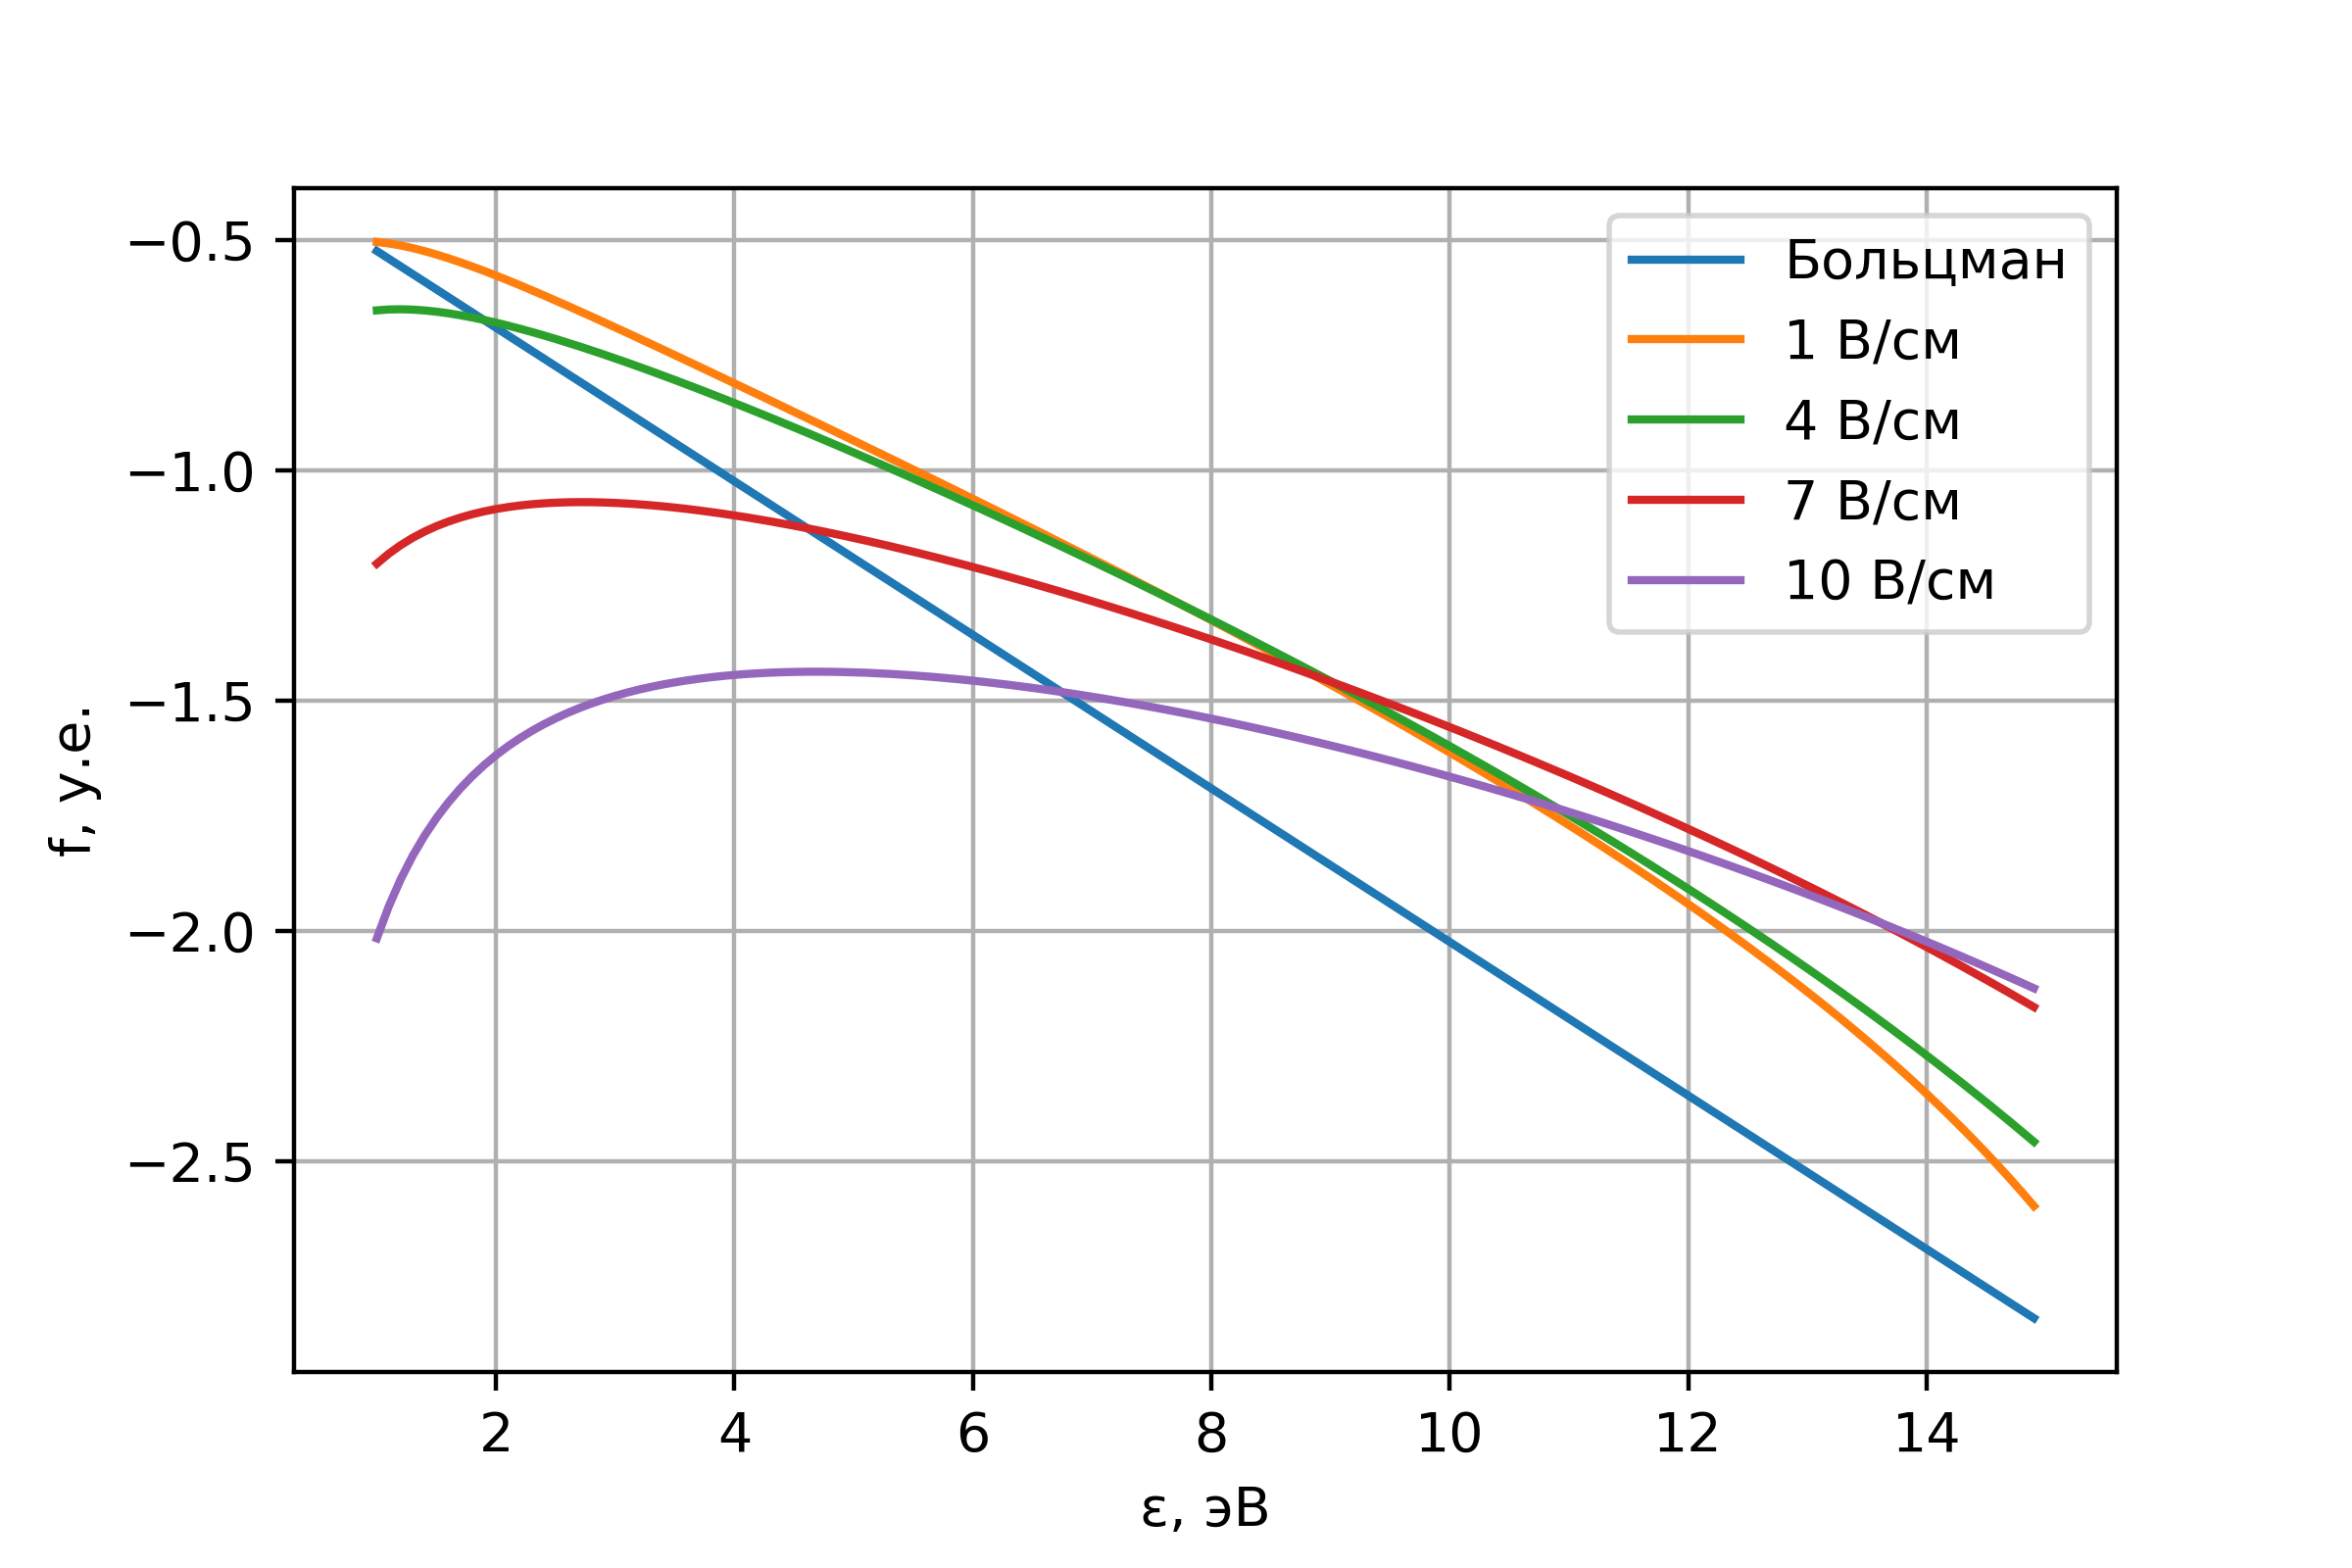
\includegraphics[width=0.49\textwidth]{figures/fig15a}
         }
         \subfloat[\label{sub:fig15b}]{
           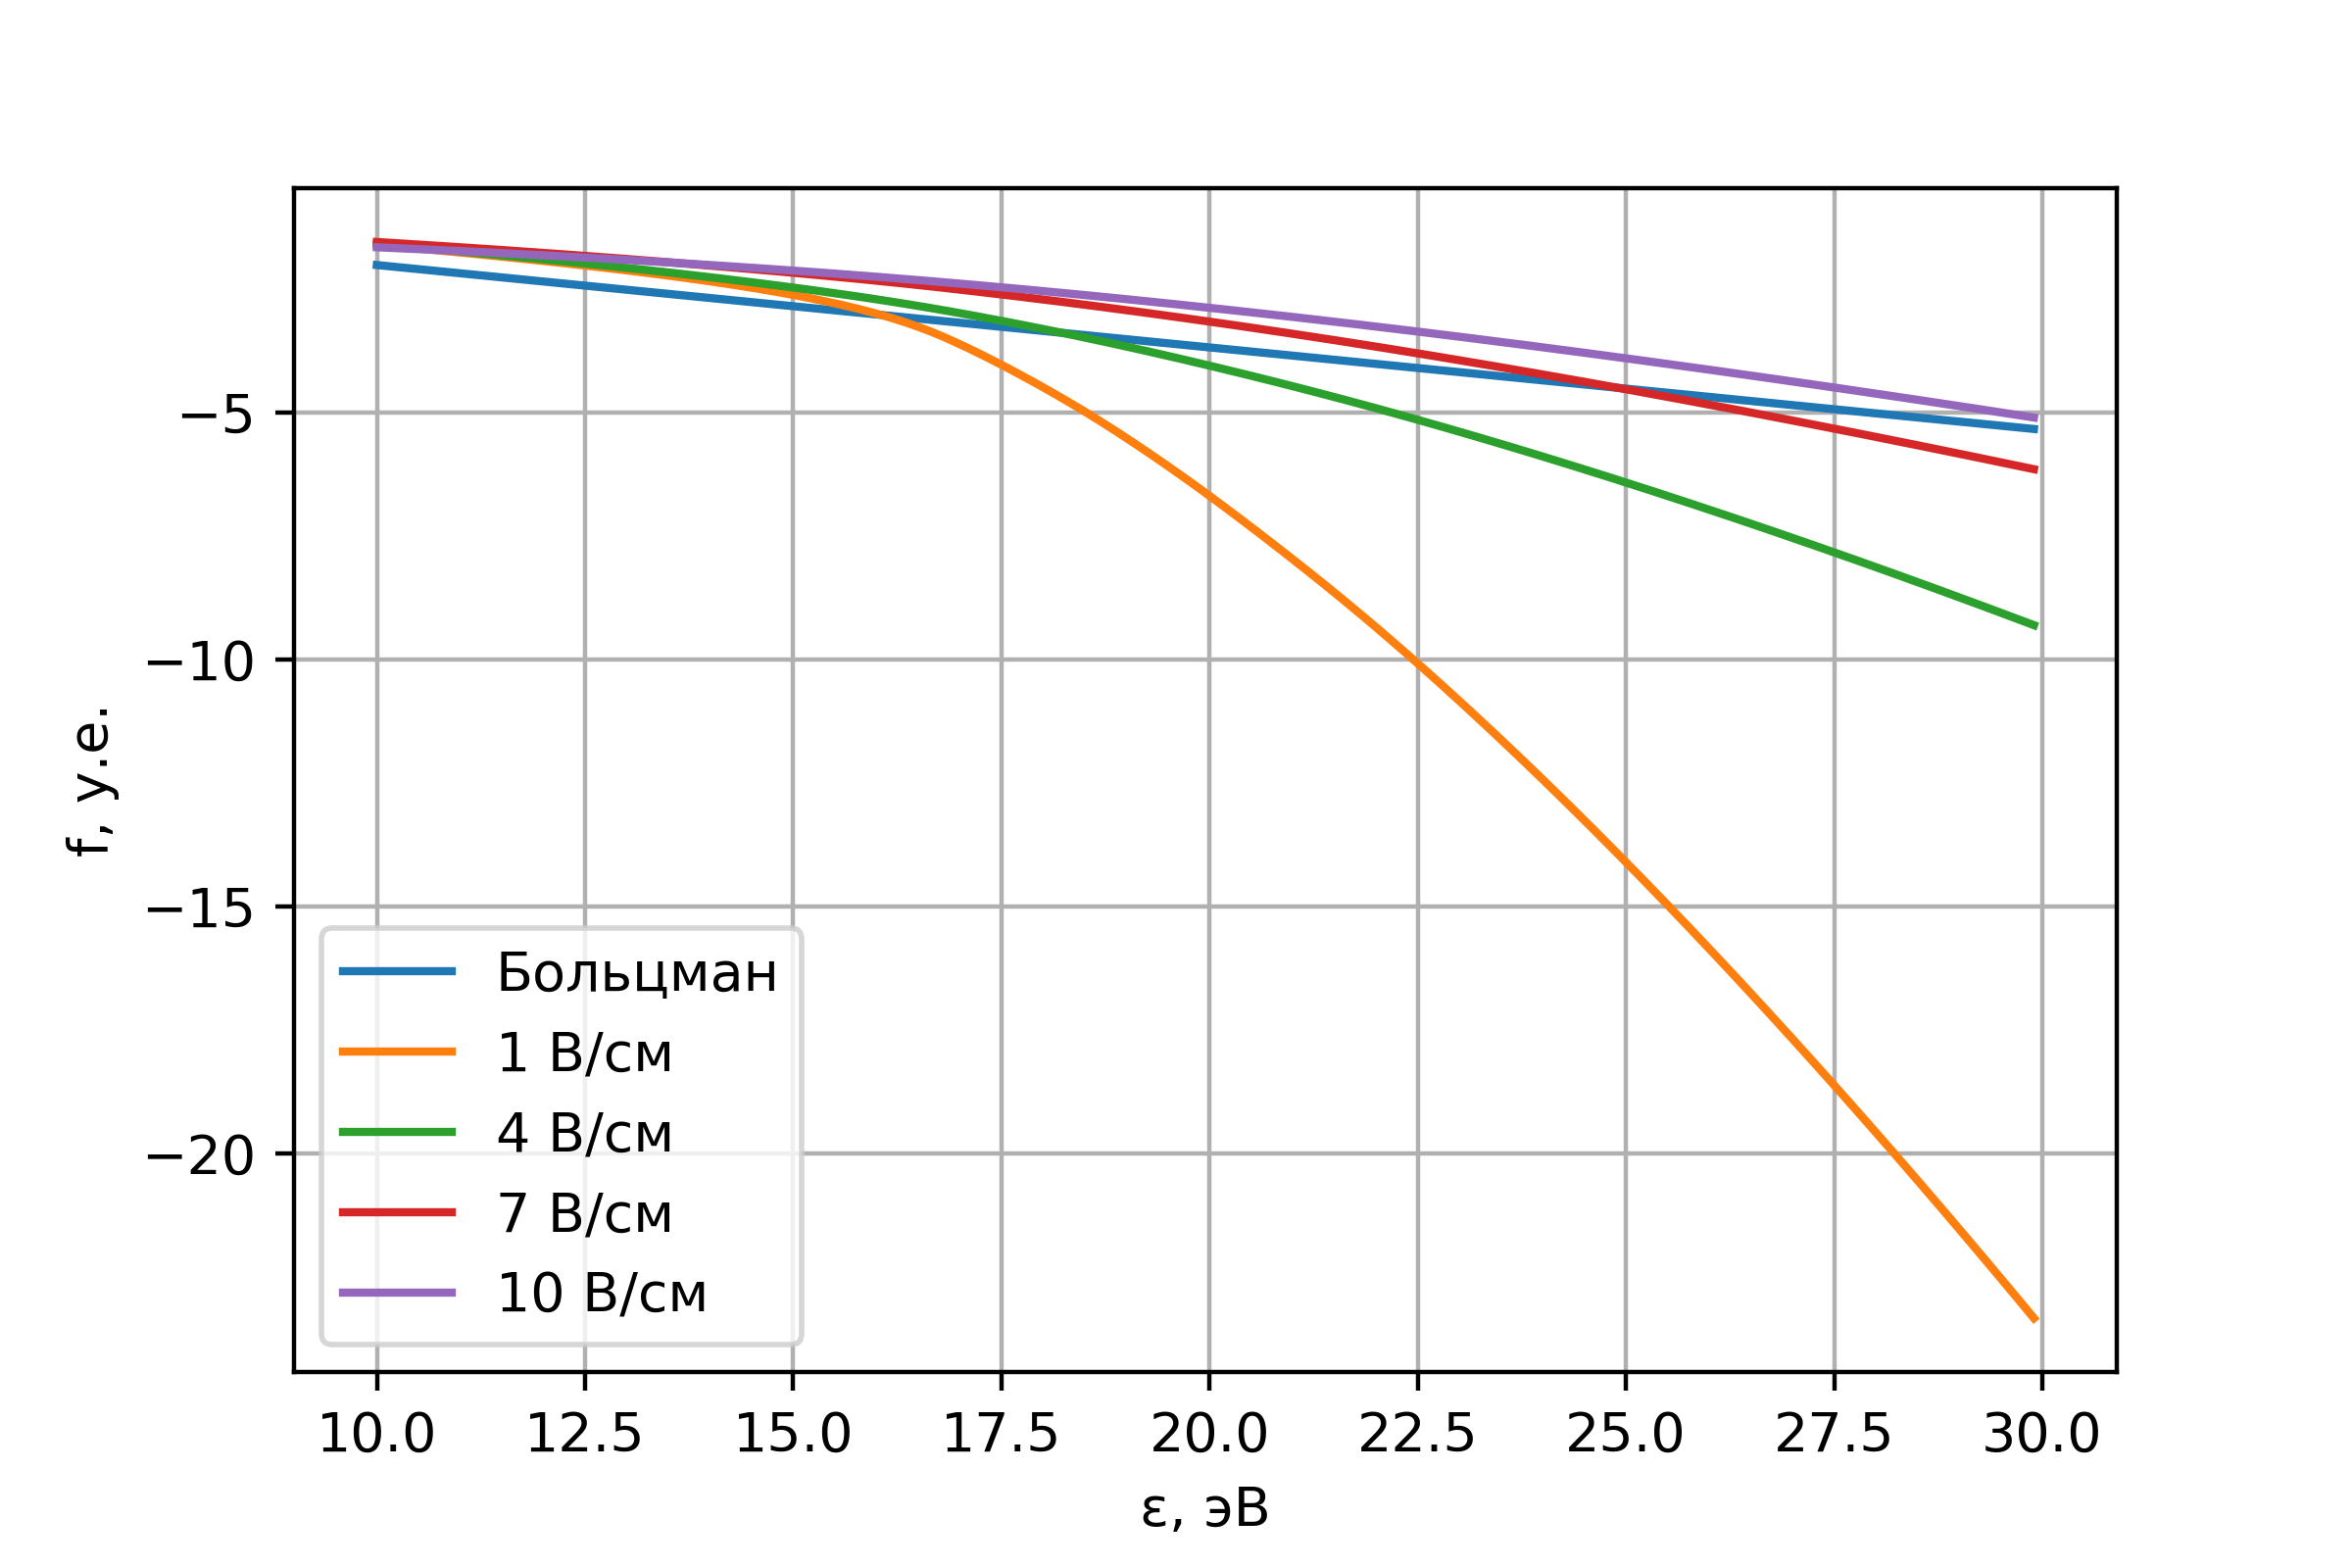
\includegraphics[width=0.49\textwidth]{figures/fig15b}
         }
         \caption{Зависимость расчетной функции распределения электронов от энергии и осевого электрического поля,
                  заданного параметрически для некоторых значений, в логарифмическом масштабе:
                  \pt(a) в диапазоне \math{1 \le \epsilon \le 15 }$~эВ, \pt(b) в диапазоне \math{10 \le \epsilon \le 30 }$~эВ;
                  также нанесено распределение Больцмана, которое использовалось в качестве начального условия (\ref{eq:start_condition}).

         }
         \label{fig:fig15}
    \end{center}
\end{figure}
\begin{equation*}
    \sigma_{18.38}(\epsilon) = \begin{cases}
    {2.024 \cdot 10^{-17} \over \epsilon + 11} \cdot \sqrt{\epsilon - 18.38 \over \epsilon}, \epsilon > 18.38 \\
    0, \epsilon \le 18.38
    \end{cases}
\end{equation}
\begin{equation*}
    \sigma_{18.6}(\epsilon) = \begin{cases}
    {1.44 \cdot 10^{-16} + 1.4 \cdot 10^{-18} \cdot \epsilon \over \epsilon + 50} \cdot \sqrt{\epsilon - 18.6 \over \epsilon}, \epsilon > 18.6 \\
    0, \epsilon \le 18.6
    \end{cases}
\end{equation}
\begin{equation*}
    \sigma_{18.71}(\epsilon) = \begin{cases}
    {3.461 \cdot 10^{-15} + 1.565 \cdot 10^{-16} \cdot \epsilon + 1.5 \cdot 10^{-18} \cdot \epsilon^2 \over (\epsilon + 37.4)(\epsilon + 27)} \cdot \sqrt{\epsilon - 18.7 \over \epsilon}, \epsilon > 18.71 \\
    0, \epsilon \le 18.71
    \end{cases}
\end{equation}
\begin{equation*}
    \sigma_{18.97}(\epsilon) = \begin{cases}
    {7.6 \cdot 10^{-17} \over \epsilon} \cdot \ln\big{(}{\epsilon \over 18.97}\big{)}, \epsilon > 18.97 \\
    0, \epsilon \le 18.97
    \end{cases}
\end{equation}
\begin{equation*}
    \sigma_{19.7}(\epsilon) = \begin{cases}
    1.8 \cdot 10^{-18} \cdot \sqrt{\epsilon - 19.7 \over \epsilon}, \epsilon > 19.7 \\
    0, \epsilon \le 19.7
    \end{cases}
\end{equation}
\begin{equation*}
    \sigma_{20.0}(\epsilon) = \begin{cases}
    1.5 \cdot 10^{-18} \cdot \sqrt{\epsilon - 20.0 \over \epsilon}, \epsilon > 20.0 \\
    0, \epsilon \le 20.0
    \end{cases}
\end{equation}
\begin{equation*}
    \sigma_{ion}(\epsilon) = \begin{cases}
    2.5 \cdot 10^{-17} \cdot {\epsilon - 21.5 \over 21.5}, \epsilon > 21.5 \\
    0, \epsilon \le 21.5
    \end{cases}
\end{equation}


Используя данные аппроксимации сечений, разностную схему, начальные и граничные условия (\ref{eq:razh_scheme}~--~\ref{eq:start_condition}),
итерационные шаги \math{\Delta \epsilon = 0.1}$~эВ и \math{\Delta t \sqrt{2 \over m} = 0.0002 }$~с~\math{\cdot}$~г^{\math{-{1 \over 2}}}$,
а также параметрически задавая осевое электрическое поле в диапазоне \math{1 \le E_z \le 10}$~эВ с шагом \math{\Delta E_z = 0.1}$~эВ,
рассчитаем ФРЭ. С графическим представлением некоторых результатов можно ознакомиться на рис. \ref{fig:fig14}.

Интенсивность свечения плазмы определенной длины волны формируется поведением ФРЭ при энергиях больше пороговой (до бесконечности),
которая имеет значение соответственно переходу для данной длины волны. Поэтому особый интерес в данной работе представляет
хвостовая часть полученной функции распределения электронов: в основном пороговая энергия для энергетических переходов неона больше
16~эВ. В обычном масштабе обнаружить на глаз поведение хвостовой части ФРЭ представляется невозможным (см.~рис~\ref{fig:fig14}):
хвостовая часть распределения Больцмана, как и остальных посчитанных распределений, сливаются между собой. Поэтому удобнее
всего перейти к логарифмическому масштабу ФРЭ (см.~рис~\ref{sub:fig15b}).

